\begin{figure}[H]
    \centering
    \includegraphics[width=.9\linewidth]{al_algo}
    \caption{A Flowchart of the Algorithm \\
    NN ... convolutional Neural Network trained to map spectra to stack and layer parameters \\
    DB ... database of FMM simulated single layers \\
    SASA ... algorithm calculating $\hat{S}_\s{Stack}$ from $\hat{S}_1$ and $\hat{S}_2$ \\
    Opt ... optimizer changing parameters to minimize the difference between the current and target spectrum \\
    layer parameters ... these include the geometry of the periodic meta surface cell and the kind of material used \\
    stack parameters ... the rotation angle of the layers to one another and the distance between \\
    new paramerters ... the Opt. only changes the continuous parameters, the discrete ones , e.g. material, remain unchanged \\
    optimization loop ... this loop is repeated until the target accuracy is reached}
    \label{fig:al:algo}
\end{figure}
